% Editable reconstructions of the three figures in the supplied PDF.
% The source PDF contains vector plots but no original plotting source.
% Coordinates below preserve its 432 bp-wide canvases, colours, and scales.
% Only \usepackage{tikz} is required; no external graphics or shell escape.
% Helvetica/Nimbus Sans replaces the PDF's embedded DejaVu Sans font.

\definecolor{EWOink}{RGB}{32,48,56}
\definecolor{EWOteal}{RGB}{0,124,131}
\definecolor{EWOrust}{RGB}{170,75,34}
\definecolor{EWOgrey}{RGB}{91,102,106}
\definecolor{EWOagent}{RGB}{98,107,117}
\definecolor{EWOgrid}{RGB}{199,205,208}
\newcommand{\PaperFigureFont}{\fontfamily{phv}\selectfont}
\tikzset{
  ewo figure/.style={x=1bp,y=1bp,line cap=butt,line join=round,
    every node/.style={anchor=base west,inner sep=0pt,outer sep=0pt,
      text=EWOink,font=\PaperFigureFont\fontsize{8.5bp}{10bp}\selectfont}},
  ewo title/.style={font=\PaperFigureFont\bfseries\fontsize{11bp}{13bp}\selectfont},
  ewo label/.style={font=\PaperFigureFont\fontsize{9bp}{11bp}\selectfont},
  ewo panel/.style={font=\PaperFigureFont\fontsize{10bp}{12bp}\selectfont},
  ewo axis/.style={draw=EWOgrey,line width=.6bp},
  ewo tick/.style={draw=EWOink,line width=.6bp}
}

\newcommand{\AttemptTimelineFigure}{%
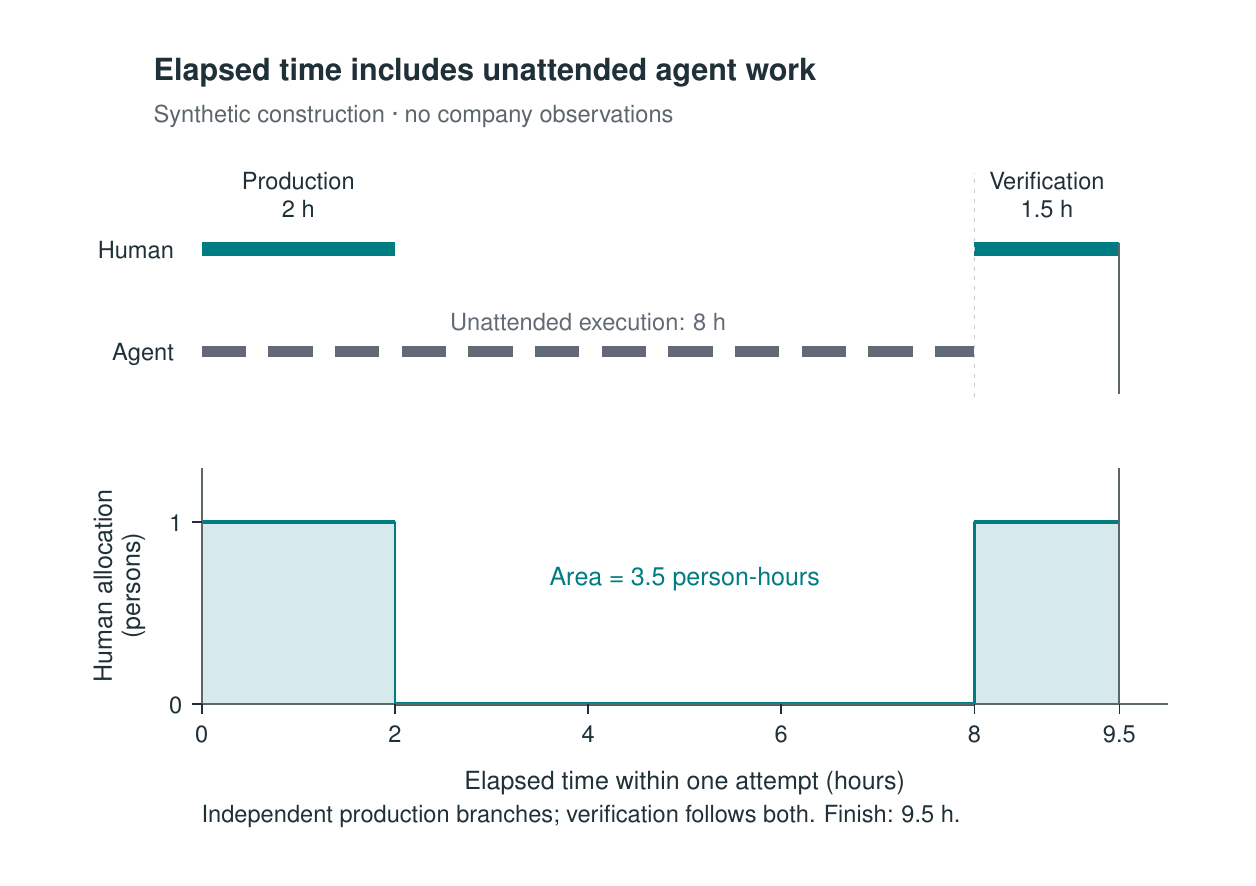
\begin{tikzpicture}[ewo figure]
  \path[use as bounding box] (0,0) rectangle (432,298.8);
  \node[ewo title] at (45.36,279.684)
    {Elapsed time includes unattended agent work};
  \node[text=EWOgrey] at (45.36,264.765)
    {Synthetic construction \textperiodcentered\ no company observations};

  % Independent branches: c_h=2 h, g=8 h, followed by v=1.5 h.
  % Both panels use x = 62.64 + 34.776 * elapsed hours.
  \node[anchor=base east] at (52.64,215.585) {Human};
  \node[anchor=base east] at (52.64,178.914) {Agent};
  \draw[EWOteal,line width=5bp] (62.64,219.007)--(132.192,219.007);
  \draw[EWOteal,line width=5bp] (340.848,219.007)--(393.012,219.007);
  \draw[EWOagent,line width=4bp,dash pattern=on 16bp off 8bp]
    (62.64,182.336)--(340.848,182.336);
  \draw[EWOgrid,line width=.7bp,dash pattern=on 1.4bp off 2.1bp]
    (340.848,165.834)--(340.848,246.51);
  \draw[EWOgrey,line width=.7bp] (393.012,166.934)--(393.012,221.207);
  \node[anchor=base] at (97.416,240.504) {Production};
  \node[anchor=base] at (97.416,230.416) {2 h};
  \node[anchor=base] at (366.93,240.504) {Verification};
  \node[anchor=base] at (366.93,230.416) {1.5 h};
  \node[anchor=base,text=EWOagent] at (201.744,189.670)
    {Unattended execution: 8 h};

  % Human allocation is one person on [0,2] and [8,9.5], zero otherwise.
  \fill[EWOteal,opacity=.16] (62.64,55.278) rectangle (132.192,120.784);
  \fill[EWOteal,opacity=.16] (340.848,55.278) rectangle (393.012,120.784);
  \draw[EWOteal,line width=.8bp]
    (62.64,55.278)--(62.64,120.784)--(132.192,120.784)--(132.192,55.278)
    (340.848,55.278)--(340.848,120.784)--(393.012,120.784)--(393.012,55.278);
  \draw[EWOteal,line width=1.5bp]
    (62.64,120.784)--(132.192,120.784)
    (132.192,55.278)--(340.848,55.278)
    (340.848,120.784)--(393.012,120.784);
  \draw[EWOgrey,line width=.7bp] (393.012,55.278)--(393.012,140.436);
  \draw[ewo axis] (62.64,140.436)--(62.64,55.278)--(410.4,55.278);
  \foreach \hour in {0,2,4,6,8,9.5}{
    \draw[ewo tick] ({62.64+34.776*\hour},55.278)--++(0,-3.5);
    \node[anchor=base] at ({62.64+34.776*\hour},41.434) {\hour};
  }
  \foreach \allocation in {0,1}{
    \draw[ewo tick] (62.64,{55.278+65.506154*\allocation})--++(-3.5,0);
    \node[anchor=base east] at (55.64,{51.856+65.506154*\allocation})
      {\allocation};
  }
  \node[ewo label,anchor=base,rotate=90] at (30.271,97.857) {Human allocation};
  \node[ewo label,anchor=base,rotate=90] at (40.359,97.857) {(persons)};
  \node[ewo label,anchor=base] at (236.52,24.716)
    {Elapsed time within one attempt (hours)};
  \node[ewo label,anchor=base,text=EWOteal] at (236.52,97.857)
    {Area = 3.5 person-hours};
  \node at (62.64,12.550)
    {Independent production branches; verification follows both. Finish: 9.5 h.};
\end{tikzpicture}%
}

\newcommand{\DetectionFigure}{%
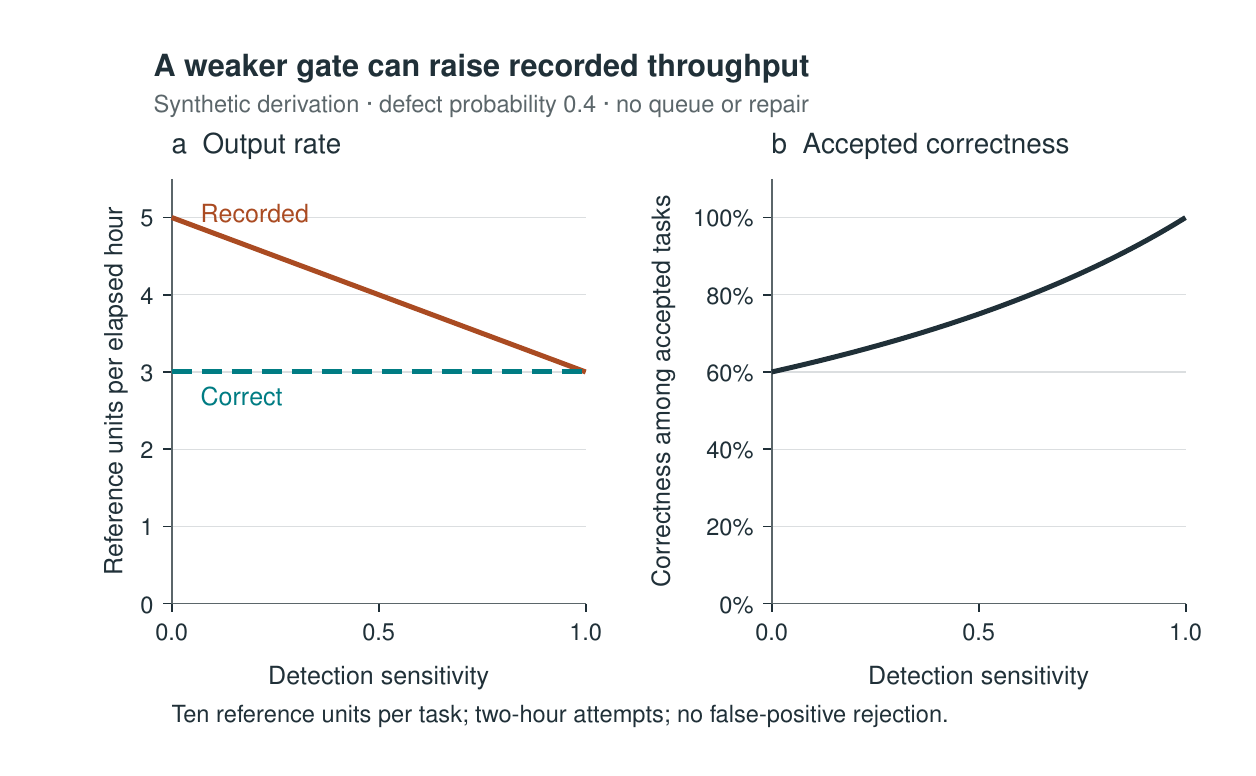
\begin{tikzpicture}[ewo figure]
  \path[use as bounding box] (0,0) rectangle (432,259.2);
  \node[ewo title] at (45.36,241.509)
    {A weaker gate can raise recorded throughput};
  \node[text=EWOgrey] at (45.36,228.769)
    {Synthetic derivation \textperiodcentered\ defect probability 0.4
     \textperiodcentered\ no queue or repair};
  \node[ewo panel] at (51.84,213.768) {a\ \ Output rate};
  \node[ewo panel] at (267.84,213.768) {b\ \ Accepted correctness};

  % Both axes: x in [0,1], left rate in [0,5.5], right fraction in [0,1.1].
  \foreach \xorigin in {51.84,267.84}{
    \foreach \step in {0,...,5}{
      \draw[EWOgrid,line width=.45bp,opacity=.65]
        (\xorigin,{51.84+27.805091*\step})--++(149.04,0);
      \draw[ewo tick] (\xorigin,{51.84+27.805091*\step})--++(-3,0);
    }
    \draw[ewo axis] (\xorigin,204.768)--(\xorigin,51.84)--++(149.04,0);
    \foreach \s/\ticktext in {0/0.0,0.5/0.5,1/1.0}{
      \draw[ewo tick] ({\xorigin+149.04*\s},51.84)--++(0,-3);
      \node[anchor=base] at ({\xorigin+149.04*\s},38.496) {\ticktext};
    }
    \node[ewo label,anchor=base] at ({\xorigin+74.52},22.778)
      {Detection sensitivity};
  }
  \foreach \step in {0,...,5}{
    \node[anchor=base east] at (45.34,{48.418+27.805091*\step}) {\step};
  }
  \foreach \step/\ticktext in {0/0,1/20,2/40,3/60,4/80,5/100}{
    \node[anchor=base east] at (261.34,{48.418+27.805091*\step}) {\ticktext\%};
  }
  \node[ewo label,anchor=base,rotate=90] at (34.059,128.304)
    {Reference units per elapsed hour};
  \node[ewo label,anchor=base,rotate=90] at (231.168,128.304)
    {Correctness among accepted tasks};

  % S^0=10, t=2, d=.4: recorded=5-2s; correct=3; rho=.6/(1-.4s).
  \draw[EWOrust,line width=1.8bp]
    plot[domain=0:1,samples=2] ({51.84+149.04*\x},{51.84+27.805091*(5-2*\x)});
  \draw[EWOteal,line width=1.8bp,dash pattern=on 7.2bp off 3.6bp]
    (51.84,135.255273)--(200.88,135.255273);
  \draw[EWOink,line width=1.8bp]
    plot[domain=0:1,samples=101] ({267.84+149.04*\x},{51.84+139.025455*(.6/(1-.4*\x))});
  \node[ewo label,text=EWOrust] at (62.273,188.919) {Recorded};
  \node[ewo label,text=EWOteal] at (62.273,123.299) {Correct};
  \node at (51.84,9.072)
    {Ten reference units per task; two-hour attempts; no false-positive rejection.};
\end{tikzpicture}%
}

\newcommand{\EffortTimeFigure}{%
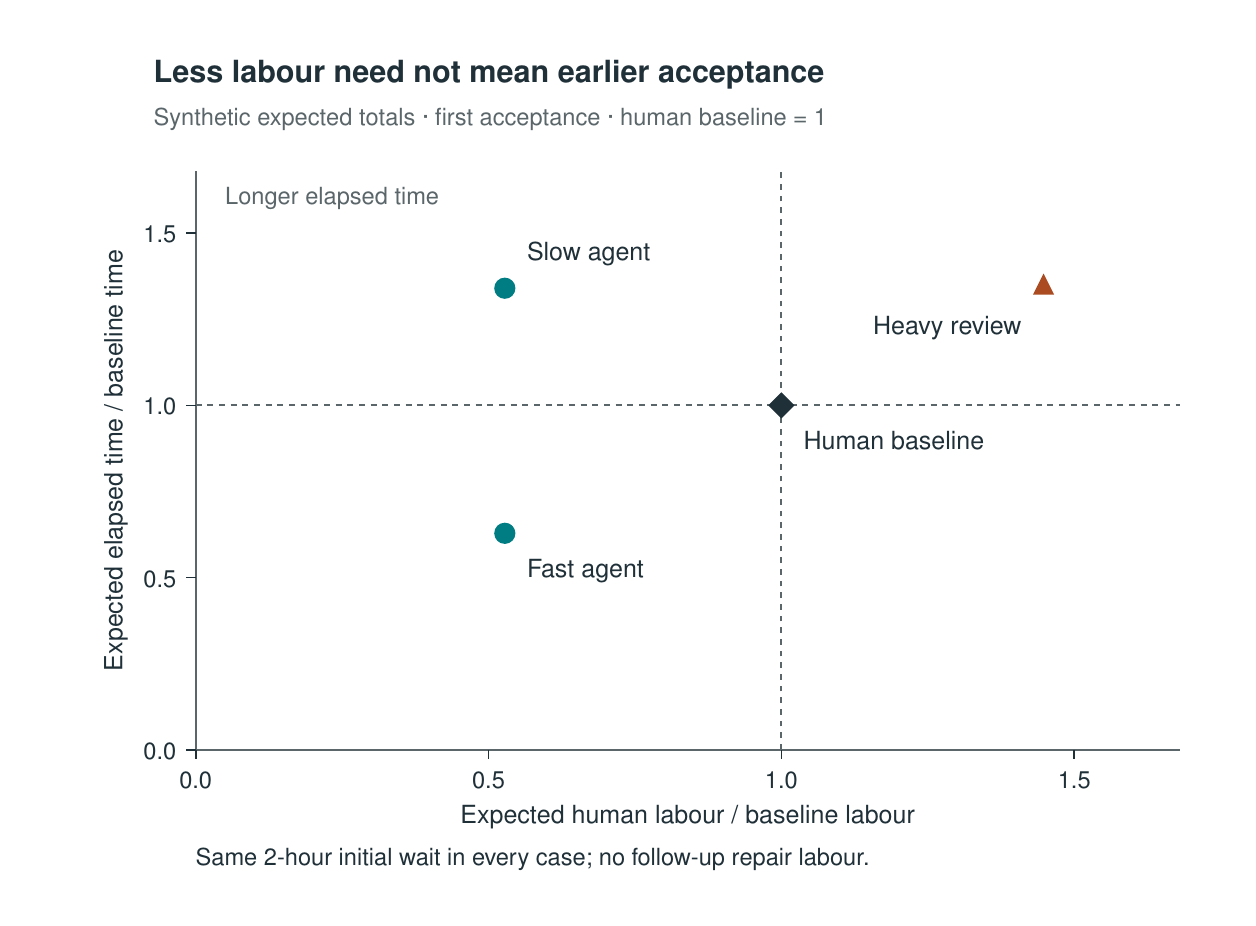
\begin{tikzpicture}[ewo figure]
  \path[use as bounding box] (0,0) rectangle (432,313.2);
  \node[ewo title] at (45.36,293.565)
    {Less labour need not mean earlier acceptance};
  \node[text=EWOgrey] at (45.36,277.855)
    {Synthetic expected totals \textperiodcentered\ first acceptance
     \textperiodcentered\ human baseline = 1};

  % Ratios of E[H^A]=h/p and E[L]=2+t/p to the human baseline.
  % Plot scales: x=60.48+210.857142857*r_H, y=53.244+123.975*r_L.
  \draw[ewo axis] (60.48,261.522)--(60.48,53.244)--(414.72,53.244);
  \foreach \value/\ticktext in {0/0.0,0.5/0.5,1/1.0,1.5/1.5}{
    \draw[ewo tick] ({60.48+210.857142857*\value},53.244)--++(0,-3.5);
    \node[anchor=base] at ({60.48+210.857142857*\value},39.400) {\ticktext};
    \draw[ewo tick] (60.48,{53.244+123.975*\value})--++(-3.5,0);
    \node[anchor=base east] at (53.48,{49.822+123.975*\value}) {\ticktext};
  }
  \draw[EWOgrey,line width=.7bp,dash pattern=on 2.1bp off 2.1bp]
    (271.337143,53.244)--(271.337143,261.522)
    (60.48,177.219)--(414.72,177.219);
  \node[ewo label,anchor=base] at (237.6,26.682)
    {Expected human labour / baseline labour};
  \node[ewo label,anchor=base,rotate=90] at (34.089,157.383)
    {Expected elapsed time / baseline time};
  \node[text=EWOgrey] at (71.107,249.471) {Longer elapsed time};

  % Baseline: h=t=7, p=.95; fast: h=t=3.5, p=.9;
  % slow: h=3.5,t=9.5,p=.9; review: h=t=8,p=.75.
  \pgfmathsetmacro{\ewobaselineH}{7/.95}
  \pgfmathsetmacro{\ewobaselineL}{2+7/.95}
  \pgfmathsetmacro{\ewofastX}{60.48+210.857142857*(3.5/.9)/\ewobaselineH}
  \pgfmathsetmacro{\ewofastY}{53.244+123.975*(2+3.5/.9)/\ewobaselineL}
  \pgfmathsetmacro{\ewoslowY}{53.244+123.975*(2+9.5/.9)/\ewobaselineL}
  \pgfmathsetmacro{\eworeviewX}{60.48+210.857142857*(8/.75)/\ewobaselineH}
  \pgfmathsetmacro{\eworeviewY}{53.244+123.975*(2+8/.75)/\ewobaselineL}
  \fill[EWOink] (271.337143,172.528584)--(276.027559,177.219)
    --(271.337143,181.909416)--(266.646727,177.219)--cycle;
  \fill[EWOteal] (\ewofastX,\ewofastY) circle[radius=3.817bp];
  \fill[EWOteal] (\ewofastX,\ewoslowY) circle[radius=3.817bp];
  \fill[EWOrust] (\eworeviewX,{\eworeviewY+3.817})
    --({\eworeviewX-3.817},{\eworeviewY-3.817})
    --({\eworeviewX+3.817},{\eworeviewY-3.817})--cycle;
  \node[ewo label] at (279.337143,161.219) {Human baseline};
  \node[ewo label] at ({\ewofastX+8},{\ewofastY-16}) {Fast agent};
  \node[ewo label] at ({\ewofastX+8},{\ewoslowY+10}) {Slow agent};
  \node[ewo label,anchor=base east] at ({\eworeviewX-8},{\eworeviewY-18})
    {Heavy review};
  \node at (60.48,11.588)
    {Same 2-hour initial wait in every case; no follow-up repair labour.};
\end{tikzpicture}%
}
